\documentclass{llncs}
\usepackage{graphicx}        % standard LaTeX graphics tool
\usepackage{booktabs} % For formal tables
\usepackage{rotating}
\usepackage{color}
\usepackage{url}

%%%%%%%%%%%%%%%%%%%%%%%%%%%%%%%%%%%%%%%%%%%%%%%%%%%%%%%%%%%%%%%%%%%%%%%%%%%%%%%%%%%%%%%%%
%\usepackage{subfigure}
%\usepackage{amsmath}
%\usepackage{makeidx}

\usepackage{rotating}

\newcommand{\bbobdatapath}{ExperimentData/KafkaEvoSpace/}

\graphicspath{{\ExperimentData}}
% rungeneric.py writes data into a subfolder of ppdata desired
\input{\bbobdatapath cocopp_commands.tex} % provide default of algname and algfolder
\renewcommand{\algfolder}{EvoSpace/}
\renewcommand{\algname}{EvoSpace}

\graphicspath{{\bbobdatapath\algfolder}}

\newcommand{\DIM}{\ensuremath{\mathrm{DIM}}}
\newcommand{\aRT}{\ensuremath{\mathrm{aRT}}}
\newcommand{\FEvals}{\ensuremath{\mathrm{FEvals}}}
\newcommand{\nruns}{\ensuremath{\mathrm{Nruns}}}
\newcommand{\Dfb}{\ensuremath{\Delta f_{\mathrm{best}}}}
\newcommand{\Df}{\ensuremath{\Delta f}}
\newcommand{\nbFEs}{\ensuremath{\mathrm{\#FEs}}}
\newcommand{\fopt}{\ensuremath{f_\mathrm{opt}}}
\newcommand{\ftarget}{\ensuremath{f_\mathrm{t}}}
\newcommand{\CrE}{\ensuremath{\mathrm{CrE}}}
\newcommand{\change}[1]{{\color{red} #1}}


\begin{document}
\sloppy

\title{A modern, event-based architecture for distributed evolutionary algorithms}
\titlerunning{A modern, event-based architecture for distributed EAs}

\author{Juan J. Merelo Guerv\'os\inst{1} \and J. Mario Garc\'ia-Valdez\inst{2}}

%
\authorrunning{Garc\'ia-Valdez, Merelo Guerv\'os}

%
%%%% list of authors for the TOC (use if author list has to be modified)
\tocauthor{ }
%
\institute{ Universidad de Granada, Granada, Spain; 
\email{jmerelo@geneura.ugr.es} \orcidID{0000-0002-1385-9741}
\and
Instituto Tecnol\'ogico de Tijuana, Tijuana BC, Mexico; 
\email{mario@tectijuana.edu.mx} \orcidID{0000-0002-2593-1114}}




\maketitle

\begin{abstract}

Cloud native applications add a layer of abstraction to the
underlying distributed computing system, defining a high-level,
self-scaling and self-managed architecture of different microservices
linked by a messaging bus. Creating new algorithms that tap these
architectural patterns and at the same time employ distributed
resources efficiently is a challenge we will be taking up in this
paper. We introduce KafkEO, a cloud native evolutionary algorithms
framework that is prepared to work with different implementations of evolutionary
algorithms and other population-based metaheuristics by using
micro-populations and stateless services as the main building
blocks; KafkEO is an attempt to map the traditional evolutionary
algorithm to this new cloud-native format. As far as we know, this is the first
architecture of this kind that has been published and tested, and is free 
software and vendor-independent, based on OpenWhisk and Kafka. 
This paper presents a proof of concept, examines its cost, and tests 
the impact on the algorithm of the design around
cloud native and asynchronous system by comparing it on
the well known BBOB benchmarks with other pool-based architectures,
with which it has remarkable functional resemblance. KafkEO results are 
quite competitive with similar architectures.


\keywords{Cloud computing, microservices, distributed computing,
  event-based systems, Kappa architecture, stateless algorithms, algorithm implementation, performance evaluation, distributed
  computing, pool-based systems, heterogeneous distributed systems,
  serverless computing, functions as a service.}
\end{abstract}

\section{Introduction}
Cloud computing is increasingly becoming the dominant way of running
the server side of most enterprise applications nowadays, the same as the browser is
the standard platform for the client side. Besides the convenience of the pay-as-you-go
model, it also offers a way of describing the infrastructure as part
of the code, so that it is much easier to reproduce results and has 
been a boon for scientific computing.
%The availability of resources only limited by your budget, and in many
%cases for free, as well as the inherent reproducibility of cloud
%deployments, has been a boon for scientific computing. 
However,
programming the cloud means that monolithic applications, that is,
applications built on a single stack of services that communicate by
layers, are no longer an efficient architectural design for scientific workflows. Cloud
architectures favor asynchronous communication over heterogeneous %favor: american
resources, and shifting from mostly sequential and monolithic 
to an asynchronously parallel architecture will also imply important
reformulation of the algorithms in order to take full advantage of these technologies.
  Cloud native applications add a layer of abstraction to the
  underlying distributed computing system, seamlessly integrating
  different elements in a single data flow, allowing the user to just focus on code and service connections. Services are {\em native} points
  in this new architecture, departing from a monolithic or even
  distributed paradigm to become a loosely collection of
services, in fact {\em microservices} \cite{microservices}, which in
 many cases are stateless, reacting to some event and
  {\em living} only while they are doing some kind of processing.
%   and not keeping state from one invocation to the next.
% redundant - Mario  
  Reactive systems not only allow massive scaling and independent deployment they are also more economical than other monolithic options.  Platform as a service (PaaS) or even Container as a Service (CaaS) approaches need to be running all
  the time in order to maintain their state, so they are paid for their size and
  time they remain active.
  At any rate, while one of the main selling points of Functions as a Service (FaaS) is their ultra-fast activation time, from our point of view their most interesting feature is the fact that they provide stateless processing. An important caveat
  of stateless processing is that algorithms must be adapted to this fact and
  turned, at least in part, into a series of stateless steps thaworking on a data stream.
    It is also taken to an atomic extreme
    with the so-called serverless architectures \cite{Varghese2018849},
    which allow vendors and users to deploy code as single, stateless
    functions, that get activated via {\em rules}, {\em triggers} or
    explicitly, reacting to events consumed from
    a message queue.
    %or bus that
    % generally reacting to events from a message queue or bus that
    % what is generated? rules are triggered and triggers fire in
    % response to events
    % Please change it to whatever you think it's the best - JJ
    %is the backbone of the application. 
    The first commercial
    implementation of this kind of architecture was released by Amazon
    with its Lambda product, to be closely followed by releases by Azure
    (Microsoft) and Google and OpenWhisk, an open source implementation
    released by IBM \cite{Baldini2016287}.

  %These architectures are {\em event-based} in the sense that program
  %flow is governed by events.
  %, which in this case are going to be simply
  %messages received by the MessageHub service.
  %These {\em events} trigger actions,
  %and actions create new message/events which start the loop all over
  %again. This is not the only mode of action in general serverless
  %architectures; however, since they define a temporal axis and make new
  %actions depend on the result of other actions, is the one that we are
  %going to choose in this paper to implement a stateless version of an
  %evolutionary algorithm.


  %There is usually no direct translation of most algorithms to this
  %architecture. This is specially true in evolutionary algorithms, who
  %rely on state, in the shape of a population, to perform their search
  %in the space of solutions. 
  %It is relatively straightforward to convert
  %an evolutionary algorithm to a stateless version by simply making a
  %{\sf generation} function $g$ that takes a population as a function
  %and returns another population. A simple serverless GA would then be
  %triggered by the creation of a initial population, and would perform
  %one or several generations in a function, returning the result to the
  %message hub and thus triggering a new action. This would be
  %functionally equivalent to a traditional, serial evolutionary
  %algorithm, and might be cheaper than a XaaS (where X can be P as in
  %platform, I as in infrastructure, C as in container or even DB, since
  %whole systems can be implemented using a database engine as a server framework) 
  %implementation since it
  %would eschew some overhead. However, it would also incur in some
  %overhead by reading and writing to the message queue and, since it
  %would be working on a single population, no scaling could be done,
  %since there would be a single pipeline.

  %There is usually no direct translation of most algorithms to this
  %architecture. This is specially true in evolutionary algorithms, who
  %rely on state, in the shape of a population, to perform their search
  %in the space of solutions.
  In this paper we want to introduce KafkEO, a serverless framework for
  evolutionary algorithms and other population-based systems. The main
  design objective is to leverage the scaling capabilities of a
  serverless framework, as well as create a system that can be deployed
  on different platforms by using free software. Our intention has
  also been to create an algorithm that is functionally equivalent to an
  %% Pool Based ??
   asynchronous, parallel, island-based, EA, which can use parallelism and at the same
  time reproduce mechanisms that are akin to migration. The island-based 
  paradigm is relatively standard in distributed EA applications, but in our case, 
  we have been using it since it allows for better parallelism
  and thus performance, at the same time it makes keeping diversity
  easier while needing fewer parameters to tune.

  We will examine the results of this framework using the first five
  functions of the Noiseless Black-Box-Optimization-Benchmarking (BBOB) testbed \cite{hansen2016coco} part of the COCO (COmparing Continuous Optimisers) platform for comparisons of real-parameter global optimisers \cite{hansen2016coco}. The framework is compared
  against another cloud-ready parallel pool based implementation.
  %The speed measurements are intended mainly as baseline,
  %since no effort has been made to optimize it.
  The
  implementation is also free software and can be downloaded from
  GitHub.
  %% TODO: Add link? 
  The rest of the paper is organized as follows. Next we present the
  state of the art in cloud implementation of evolutionary algorithms,
  to be followed in section \ref{sec:methods} by an introduction to the
  serverless architecture we will be using as well as our mapping of the
  evolutionary algorithm to it. Section \ref{sec:res} will present the
  result of performing experiments with this proof of concept; finally
  in section \ref{sec:con} will discuss the results, present conclusions
  and future lines of work.


  \section{State of the art}
  In general, scientific computing has followed the trends of the
  computing industry, with new implementations published almost as soon
  as new technologies became commercially available, or even
  before. There were very early implementations of evolutionary
  algorithms on transputers \cite{voigt1990modelling}, the world wide
  % transputers, had to google that
  % you're too young, man - JJ
  web \cite{chong:1999:jDGPi} and the first generation of cloud
  services
  \cite{DBLP:journals/corr/abs-1105-6205,de2017parallel,salza2017ccube}. %Evolutionary
  %algorithms are population-based algorithms, so it is relatively easy
  %to create a parallel implementation by just splitting populations, as
  %long as there is a way for those populations to interchange some
  %individuals and leverage the use of many different machines. In
  %general, besides, one of the most time-consuming steps in an
  %evolutionary algorithm is evaluation, so as long as you can compute
  %fitness in parallel, you can obtain a certain amount of speed up.
  However, every new computing platform has its own view of computing, and in many cases that has made evolutionary algorithms move in new directions in order to make them work better in that platform while keeping the spirit of
  bio-inspiration. For instance, most evolutionary algorithms work in a
  synchronous way; although there were very early efforts to create
  asynchronous EAs \cite{coleman89}, in general
  generations proceed one after the other and migration happens in
  all islands at the same time. However, this mode of working does not
  fit well with architectures that are heterogeneous and dynamic, which
  is why there have been many efforts from early
  on to adapt EAs to this kind of substrate
  \cite{Jini:FEA2000,zorman2002creation,baugh2003asynchronous}.
  %This last one creates an asynchronous, parallel system that is {\em functionally equivalent} to a sequential one by {\em unrolling} operations so
  %that they happen in parallel as long as there is no dependence between
  %them; multiple generations occur at the same time with every operation
  %using data that is available at every particular moment.
  %\cite{Jini:FEA2000} and \cite{zorman2002creation} explicitly
  %follow two completely different, and opposed, approaches to the
  %adaptation of an EA to a heterogeneous substrate. While the former
  %tends towards finer grain by distributing every particular operation
  %to different Jini services, the latter uses a pool-based approach to
  %create island-like structures, creating again a system that, even
  %leveraging the capabilities of the architecture in a much better way,
  %does not advance the  structure of an EA in any new way.

  This kind of internet-native applications later on transitioned to
  using Service-Oriented Architectures (SoA) \cite{Papazoglou2007}. While monolithic, that is,
  including all services in a single computing node and application, SoA
  were better adapted to heterogeneous environments by distributing
  services across a network using standard protocols. Several authors
  implemented evolutionary algorithms over them
  \cite{garcia2013service,munawar2010design,6955331}. However, scaling
  problems and the extension of cloud deployment and services had made
  this kind of architectures decline in popularity.
%  \cite{Varghese2018849}. Too big citation

  In general, frameworks based in SoA also tried to achieve functional equivalence with parallel
  or sequential versions of EAs. There is the same tension between
  functional equivalence and new
  design in new, cloud based approaches to evolutionary
  algorithms. 
  %TODO: The previous should be improved, is very important. 
  Salza and collaborators \cite{salza2017ccube,de2017parallel} explicitly
  and looking to optimize interoperability claim that there is very
  little need to change ``traditional'' code to port it to the cloud,
  implicitly claiming this {\em functional equivalence} with
  sequential evolutionary algorithms.
  % Not that important or related? - Mario
  %Other contemporary systems such as
  %\cite{10.1007/978-3-319-32149-3_46} use Spark to evaluate, in
  %parallel, fitness for different machine learning models;
  %Vianna de Oliveira and Coelho \cite{de2015scalable} use Hadoop for evolutionary k-means clustering,
  %obtaining good speedups; in this last case, it uses a problem-specific
  %way of distributing tasks, without resourcing to a change of the
  %evolutionary algorithm itself.

  % Yes! we got to the chase 
  Besides these implementations using well known cloud services, there are new computation models for evolutionary algorithms
  that are not functionally equivalent to a canonical EA, but have
  proved to work well in these new environments. Pool based EAs,
  \cite{bollini1999distributed}, with a persistent population that can
  be tapped to retrieve single individuals or pools of them and return
  evaluated or evolved sub-populations, have been used for new
  frameworks such as EvoSpace \cite{García-Valdez2015}, and proved to be
  able to accommodate all kinds of ephemeral and heterogeneous
  resources.

  In the serverless, event-based architectures we are going to
  be targeting in this paper, there has been so far no work that we know
  of. Similar setups including microservices have been employed by Salza et
  al. \cite{salza2017ccube}; however, the proposed serverless system adds a layer of abstraction to event-based queuing systems such as the one employed
  by Salza by reducing it to functions, messages and rules or
  triggers. We will explain in detail these architectures in the next
  section.

  % Moved here to make it go to the top of page 3
  \begin{figure*}[h!tb]
    \centering
  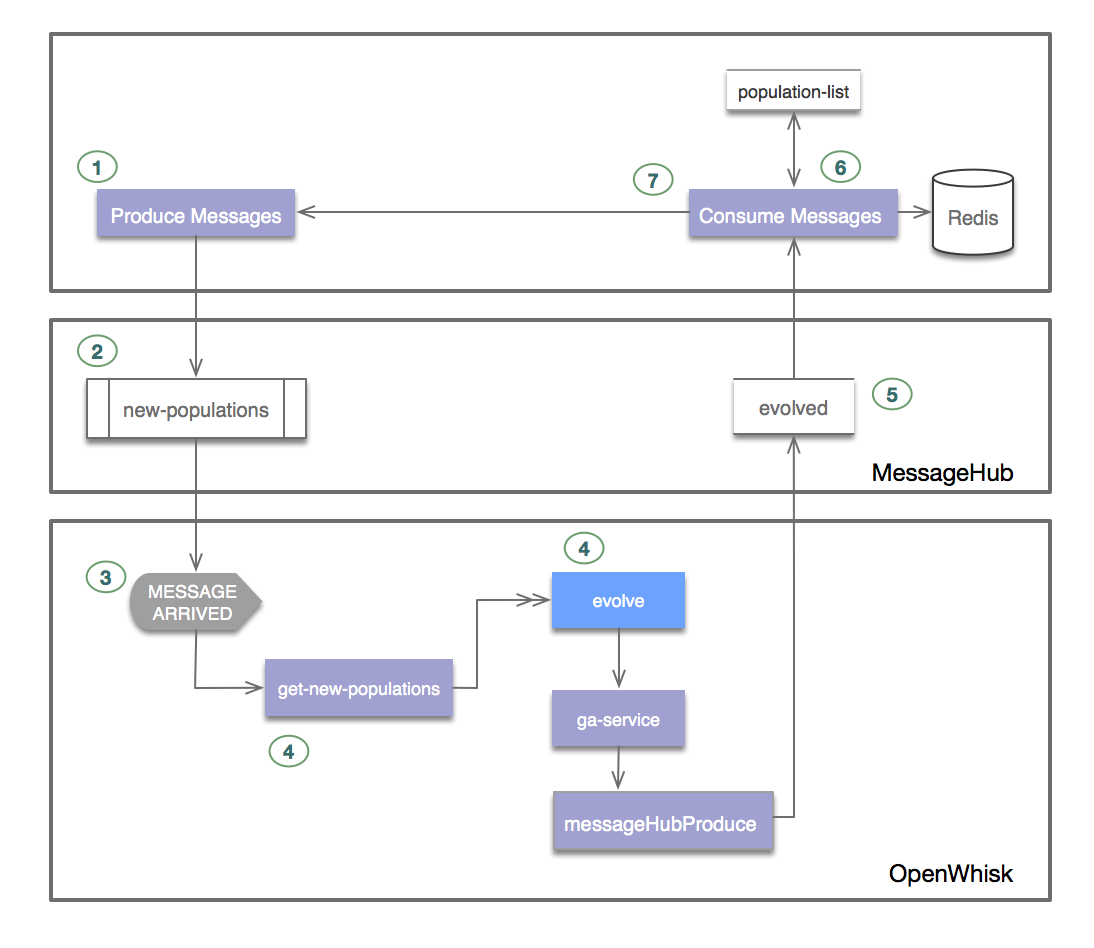
\includegraphics[width=0.75\textwidth]{img/kafka.png}
  \caption{Chart showing the general picture of the layers of a
    serverless architecture, including the messages and services that
    constitute KafkEO, with labels indicating message
    routes and the software components used for every part.}
  \label{fig:kafkeo}
  \end{figure*}
  
  \section{Event-based architectures and implementing evolutionary
    algorithms over them}
  \label{sec:methods}
  %
  \begin{figure*}[h!tb]
  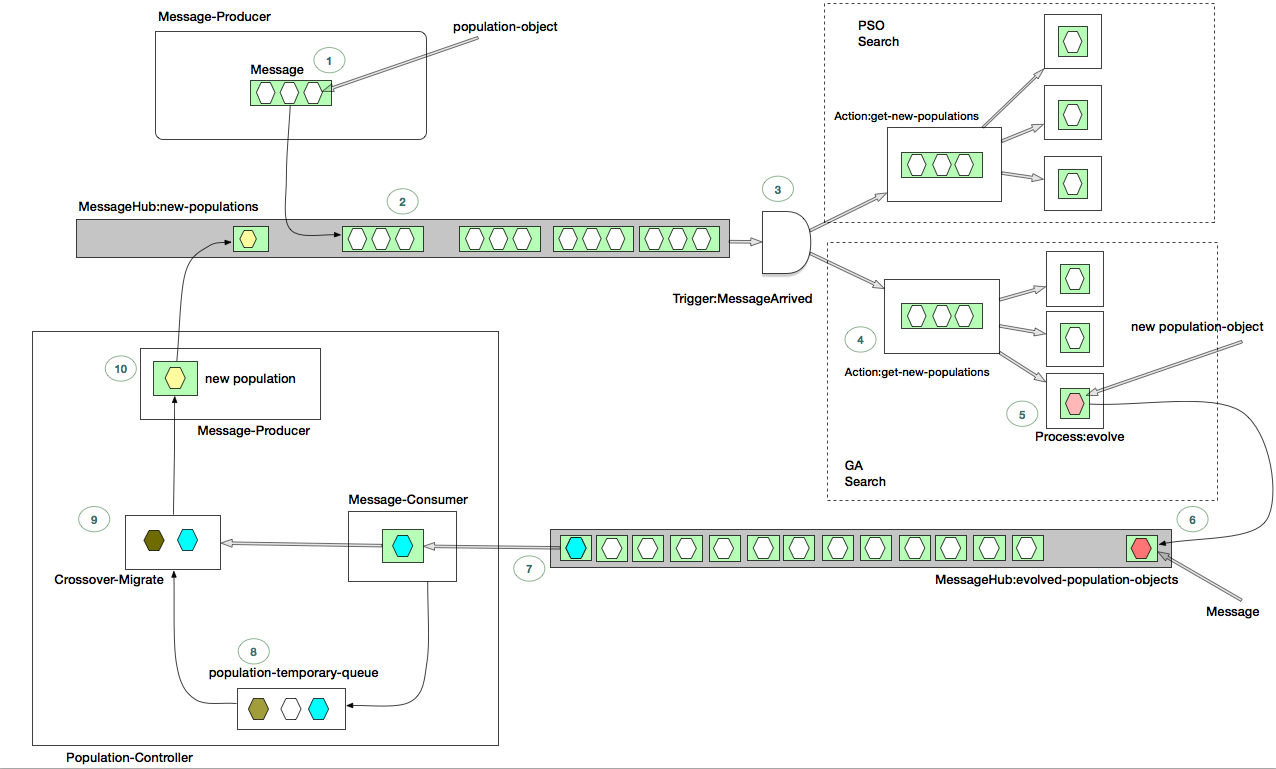
\includegraphics[width=0.75\textwidth]{img/kafkEO.png}
  \caption{A flow diagram of KafkEO, showing message routes, MessageHub
    topics and the functions that are being used.}
  \label{fig:kafkeo2}
  \end{figure*}
  % Talked about this earlier: - M
  %The creation of virtualization and isolation mechanisms at many
  %different levels and the consequent granularization of architectures
  %has led to systems that are asynchronous and loosely coupled in what
  %is generally called a microservice architecture. 
  
  %These microservice
  Microservice architectures share the common trait of consisting of several services with a single concern, that is, providing a single processing value,
  in many cases stateless, and coupled using lightweight protocols such
  as REST and messaging buses that carry information from every service
  to the next. In this case, we are going to be using IBM's BlueMix
  service, which includes OpenWhisk as a serverless framework and
  MessageHub, a vendor implementation of the Kafka messaging
  service; this last one gives name to the framework we are presenting, called KafkEO (EO stands for Evolving Objects).

  The main reason for choosing OpenWhisk and Kafka is availability of
  resources, but also the fact that all parts of the implementation are open source and can be deployed in desktop machines or other cloud providers by changing the configuration. It is also a good practice to implement free
  software using free software, making it widely available to the
  scientific community.
  % to create their own versions or to adapt it to their own problems.

  The layers and message flow in the application are shown in Figure
  \ref{fig:kafkeo}, which also includes the evolutionary components. We
  will focus for the time being in the general picture: a serverless
  architecture using a messaging service as a backbone, which in this case
  takes the shape of the Kafka/MessageHub service. 
  These messages are produced and
  consumed by a service, which can also store them in an external database
  for their later use; in general, messaging systems are configured to
  keep messages only for a certain amount of time, and they disappear
  after that. Messaging queues are organized in {\em topics} and every
  topic uses a series of {\em partitions}, which can be increased for
  bigger throughput; the
  functions, hosted in OpenWhisk, execute {\em actions} triggered by the
  arrival of new messages; these actions also produce new messages that
  go back to the MessageHub to continue with the message loop. If all
  this is hosted in a cloud provider, as it is the case, the MessageHub
  service will be charged according to a particular cost
  structure, with partitions taking the most part of
  the cost, while messages have a relatively small impact.

  The evolutionary algorithm mapped over this architecture is 
  represented in Figure \ref{fig:kafkeo2}. The main
  design challenge is to try and map an evolutionary algorithm to a
  serverless, and then stateless, architecture. That part is done in
  points 1 through 5 of Figure \ref{fig:kafkeo2}. The beginning of the
  evolution is triggered from outside the serverless framework (1) by
  creating a series of Population objects, which we pack (2) to a message in the
  {\sf new-populations} {\em topic}. Population objects are the equivalent to islands or samples in EvoSpace. If Population object is a self-contained population of individuals, represented as a JSON structure. 
    
  The arrival of a new population
  package sets off the {\sf MessageArrived} trigger (3), that is bound to
  the actions that effectively perform a small number of generations. In this case we give as an example a GA and a PSO algorithms, 
  although only the GA has been implemented 
  for this paper. Any number of GA algorithms ({\em actions}) can be triggered in parallel by the same message, and new actions can be triggered while others are still working; this phase is
  then self-scaling and parallel by design.

  Population objects are extracted from the message and, for each, a call to
  an {\em evolve} process is executed in parallel. The {\em evolve} process
  consists of two sequential {\em actions} (5), first, the {\em GA Service} function that
  runs a GA for a certain number of generations, producing a new evolved
  object, which is then sent to the second action called {\em Message Produce}
   responsible of sending the object to the {\sf evolved-population-objects} 
   message queue.  The new Population object (6) includes
   the evolved population and also metadata such as a flag indicating
  whether the solution has been found, the best individual, and information
  about each generation. With this metadata a posterior analysis of the experiment
  can be achieved or simply generating the files used by the BBOB Post-processing scripts.

  This queue is polled by a service outside the serverless framework, called
  {\sf Population-Controller}. This service needs to be stateful, since it implements a buffer that needs to wait until several populations are ready to then mix them (in step \#9 in Figure \ref{fig:kafkeo2}) to produce a new population, that is the result of selection
  and crossover between several populations coming from the {\sf
    evolved-population-objects} message queue. Eventually, these mixed
  populations are returned to the initial queue to return to the {\em
    serverless} part of the application. Another task of the 
    {\sf Population-Controller} is to start and stop the experiment. The service must
    keep the number of Population objects received, then after
    a certain number is reached, the controller stops sending new messages to the
    {\sf new-populations} {\em topic}. It is important to note, that because of
    the asynchronous nature of the system, several messages could still
    arrived after the current experiment is over. The controller must only
    accept messages belonging to the current process.
  % consists essentially on a single function, a single topic
  % in the MessageHub and a single kind of message, which includes a whole
  % population along with metadata. The function performs a series of
  % generations on the population, using a canonical algorithm with
  % mutation and crossover. If it finds the solution, in our case, the
  % minimum fitness, it sets a flag indicating it has found it so that it
  % propagates to different instances of the population; in any case, it
  % sends the whole evolved population as a message to the MessageHub, to
  % be propagated to the other instantiations on the function.

  %This would be functionally equivalent to a sequential algorithm except
  %for the fact that, between two calls to the {\sf get-new-populations}
  %function, several
  %population-messages have been received in the message queue. In fact,
  %every call the {\sf Crossover-migrate} function receives several
  %populations, which
  %have to be merged to generate several new populations. 
  This {\em merging} step
  before starting evolution takes the place of the {\em migration} phase
  and allows this type of framework to work in parallel, since several
  instances of the function might be working at the exact same time; the
  results of these instances are then received back by every one of the
  instances.

  In fact, this kind of system would be more functionally equivalent to
  a pool-based architecture \cite{bollini1999distributed}, since the
  queue acts as a pool from where populations are taken and where
  evolved populations return. Actually, the pool becomes a {\em stream}
  in this case, but in fact the pool also evolves, changing its
  composition, and has a finite size just like the pool. Since
  pool-based architectures have already proved they work with a good
  performance, we might expect this type of architecture, being
  functionally equivalent, to be at least just as efficient and the
  latter, and better adapted to a cloud-native application.

  In this phase where we are creating a proof of concept, there is a
  single instance of this part. For the time being, it has not been
  detected as a bottleneck, although eventually, when the number of
  functions are working in parallel, it might become one. There are
  several options for overcoming this problem, the easiest of which is
  to add more instances of this {\sf Population-controller}. These
  instances will act in parallel, processing the message queue at
  different offsets and contributing to population diversity. This will
  eventually have its influence in the results of the algorithm, so it
  is better left as future work.

  Since we are running just a few functions, the amount of code of KafkEO
  is quite small compared with other implementations. We use DEAP for
  all the evolutionary functions, which are written in Python and
  released in GitHub under the GPL license.

  \section{Experiments and results}
  \label{sec:res}
  
  In this section we compare the performance of KafkEO against an implementation of
  the EvoSpace \cite{GValdez2015} pool-based architecture, using the first five
  functions of the Noiseless BBOB testbed \cite{hansen2016coco}, 
  which are real-parameter, single-objective, separable functions, namely: Sphere,,  ellipsoidal, which is highly multimodal,  Rastrigin,  Buche-Rastrigin,  and the purely lineal function called linear  slope. It is expected that the two algorithms achieve similar results as
  they are functionally equivalent. The EvoSpace implementation follows the
  basic EvoSpace model in which EvoWorkers asynchronously interact with the
  population pool by taking samples of the population to perform a standard
  evolutionary search on the samples, to then return newly evolved solutions back
  to the pool.

  EvoWorkers were implemented in Python with the same code as KafkEO and using
  DEAP \cite{fortin2012deap} for the GA service function. The code is in the
  following GitHub repository: \url{https://hidden.com}. Before each
  experiment, a script initializes the population on the server, creating the
  number of individuals specified by the {\em Pool Size} parameter, this
  size depends on the dimension of the problem according to the BBOB testbed.
  When starting each EvoWorker, the following parameters are used: first, the
  {\em Sample Size} indicating the number of individuals the worker would take
  from the server on each interaction, then the {\em Iterations per Sample}
  parameter specifies the number of generations or iterations the worker algorithm
  will run before sending back to the server the resulting population. Finally,
  the number of times an  EvoWorker will take, evolve and return a sample, is
  indicated by the {\em Samples per Worker} parameter.
   The number of EvoWorkers instantiated for the experiment 
   is given by the {\em GA Workers} parameter.  The EvoSpace parameters
  are shown in Table \ref{tab:params:evoworkers}.
   These parameters are set for
  each dimension and they indicate the effort in number of evaluations. In both
   experiments the maximum number of evaluations is $10^5 \cdot D$. For instance,
   for $D = 2$, the maximum number of evaluations is $200,000$ which is 
   obtained by multiplying
    the parameters int the first column of Table \ref{tab:params:evoworkers}: $50 \cdot 100 \cdot 20 \cdot 2$. Also both algorithms limit the search space to $[-5,5]^D$.

  \begin{table}
    \small
    \caption{EvoWorker setup parameters,
      % including the number of dimensions of the
      % benchmark functions, sample size, which is the size of the block
      % of individuals taken and dropped back in the pool, as well as the
    %   number of actual workers used and samples per worker.
    }
    \label{tab:params:evoworkers}
    \centering
    \small
    \begin{tabular}{|l|c|c|c|c|c|c|}
      \hline
      Dimension & 2 & 3 & 5 & 10 & 20 & 40\\ \hline
      Iterations per Sample  & 50 & 50 & 50 & 50 & 50 & 50\\ \hline
      Sample Size  & 100 & 100 & 100 & 200 & 200 & 200 \\ \hline
      Samples per Worker & 20 & 30 & 25 & 25 & 25 & 25  \\ \hline
      GA Workers & 2 & 2 & 4 & 5 & 8 & 16  \\ \hline
      Pool Size & 250 & 250 & 500 & 1000 & 2000 & 4000  \\ \hline
    \end{tabular}
  \end{table}

  On the other hand, the parameters used for KafkEO are shown in Table
  \ref{tab:params:kafka}. Every function runs an evolutionary algorithm
  for the shown number of iterations and with the population size also
  shown. The number of initial messages act as an initial trigger, being
  thus equivalent to the number of parallel functions or workers; this is the
  tunable parameter used for increasing performance when the problem
  dimension, and thus difficulty, increases; the population size is also
  increased, so that initial diversity is higher. Please note that every
  population is generated randomly, so that the population size would
  have to be multiplied by the number of initial messages to get to the
  initial population involved in the experiment. The effort is limited by the
  maximum number of messages consumed by the {\em Population-Controller} from
   the  {\sf evolved-population-objects} message queue. The maximum number is
    calculated by multiplying the {\em  Maximum Iterations} and {\em Initial
   Messages} parameters. Again for a $10^5 \cdot D$ maximum number of evaluations.

  \begin{table}
    \small
    \caption{KafkEO parameters for the BBOB benchmark. Dimensions are 
    the independent variable, the rest of the parameters are changed to 
    adapt to the increasing difficulty. }
    \label{tab:params:kafka}
    \centering
    \small
    \begin{tabular}{|l|c|c|c|c|c|c|}
      \hline
      Dimension & 2 & 3 & 5 & 10 & 20 & 40\\ \hline
      Iterations & 50 & 50 & 50 & 50 & 50 & 50\\ \hline
      Population Size  & 100 & 100 & 100 & 200 & 200 & 200 \\ \hline
      Initial Messages & 2 & 2 & 4 & 5 & 8 & 16  \\ \hline
      Maximum Iterations & 2 & 2 & 4 & 5 & 8 & 16  \\ \hline
    \end{tabular}
  \end{table}

  The evolutionary algorithm implemented in KafkEO used the same code,
  also delegating the evolutionary operations to the standard DEAP
  library, written in
  Python \cite{fortin2012deap},
%  The parameters for the evolutionary algorithm were fixed and
%  are shown in Table \ref{tab:GAparams}.
  using 12 for tournament size, a gaussian mutation sith sigma = 0.05 and a probability between 0.1 and 0.6, plus two point crossover with probability between 0.8 and 1; these are the default parameters.  
  % These parameters have been
  % chosen as the usual, and default, setup in any experiment, without
  % making any attempt to adapt it to this particular flavor of the
  % algorithm.
  In particular, the tournament size injects a high selective
  pressure which is known to decrease diversity. The system also allows
  to set different parameters for every instance; in this proof of concept
  only two parameters were randomly set, {\em Mutation Probability}
  uniformly random in the $[.1,.6]$ range, and {\em Crossover
    Probability} random on $[.8,1]$. This is one deviation from the
  standard evolutionary algorithm, but has been proved in the past to
  provide good results without needing to fine tune different
  parameters \cite{tanabe2013evaluation}.

  %Besides, despite the
  %system allowing for different parameters for every instance, even
  %working in parallel, or random parameters for every instantiation, we
  %have made no attempt to use this feature in this proof of concept
  %stage of the algorithm.
  % Yes we did, Mutation Probability random in the range: [.1,.6] and
  % Crossover Probability& [.8,1]  \\ \hline
  % I didn't know that... Maybe we should have left it fixed - JJ

  The experiments using the above described framework were performed
  during the month of January using a paid IBM BlueMix subscription. The
  totality of experiments costed about \$12. Most of the cost is due to
  the MessageHub {\em partitions}, that is, the hosted messaging service
  itself. The amount paid for the messages in the BlueMix platform
  is less than one dollar in total; messages are paid by the hundreds of
  thousands delivered, and are actually not the most expensive part of the
  implementation of the algorithm.
  Partitions are
  essential for a high throughput; a messaging queue will be able to
  process as many messages as the partitions are able to get through in
  parallel; this means that cost will scale with the number of messages
  in a complex way, not simply linearly, and design decisions will have
  to be taken. The baseline is that the best option is to maximize the
  number of messages that can be borne by a particular partition, and
  try to minimize the number of partitions to avoid scaling costs.

  \begin{figure*}[h!tb]
  \begin{tabular}{l@{\hspace*{-0.025\textwidth}}l@{\hspace*{-0.025\textwidth}}l@{\hspace*{-0.025\textwidth}}l}
  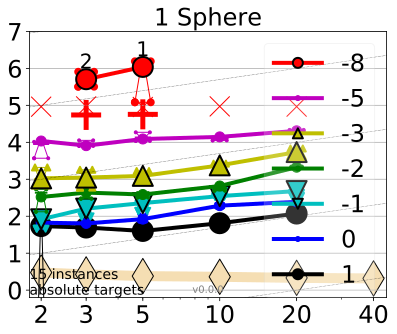
\includegraphics[width=0.266\textwidth]{ppfigdim_f001}&
  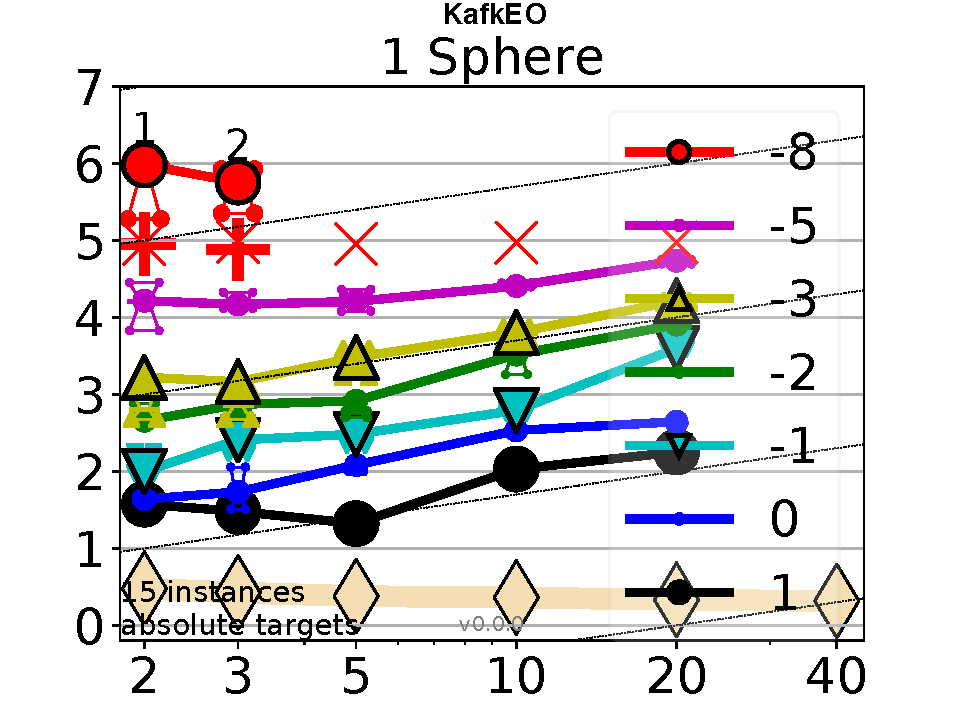
\includegraphics[width=0.266\textwidth]{ppfigdim_f006}&
  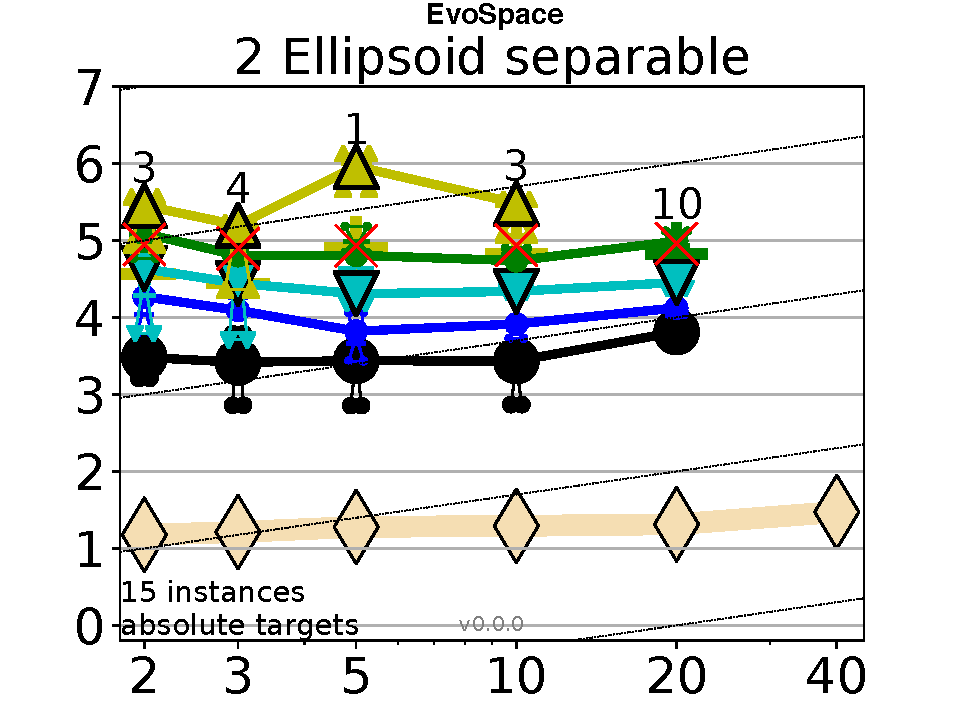
\includegraphics[width=0.266\textwidth]{ppfigdim_f002}&
  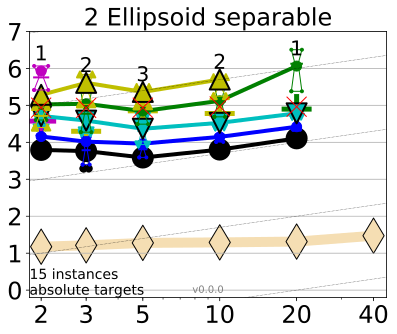
\includegraphics[width=0.266\textwidth]{ppfigdim_f007}\\
  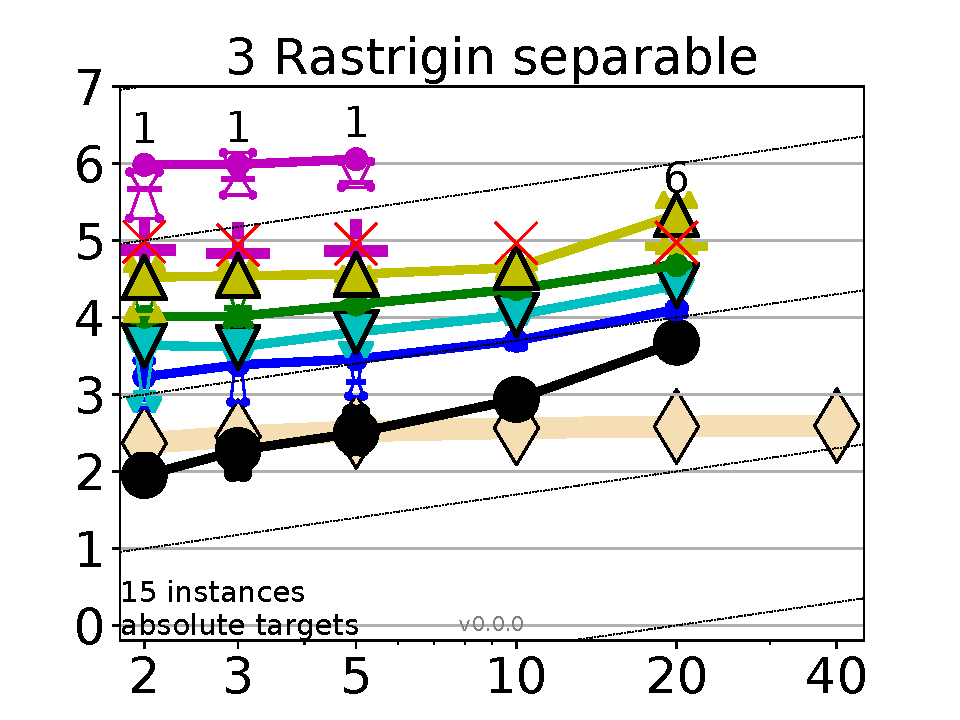
\includegraphics[width=0.266\textwidth]{ppfigdim_f003}&
  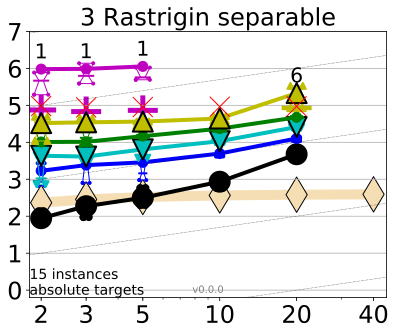
\includegraphics[width=0.266\textwidth]{ppfigdim_f008}&
  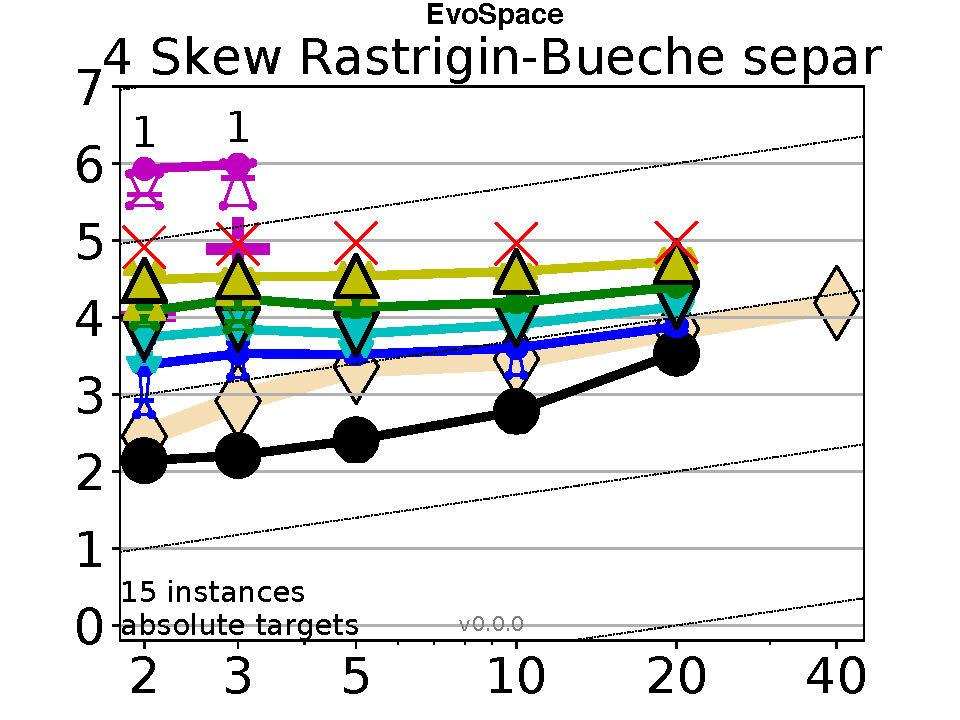
\includegraphics[width=0.266\textwidth]{ppfigdim_f004}&
  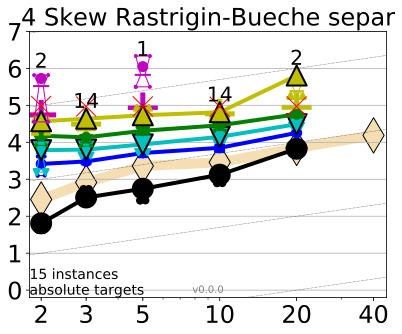
\includegraphics[width=0.266\textwidth]{ppfigdim_f009}\\
  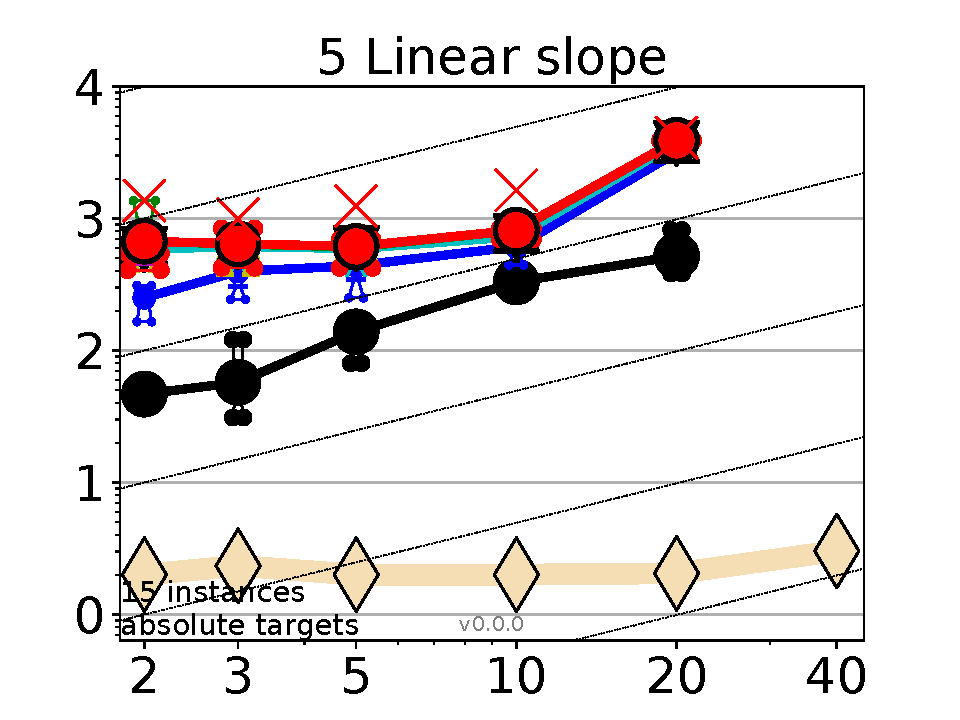
\includegraphics[width=0.266\textwidth]{ppfigdim_f005}&
  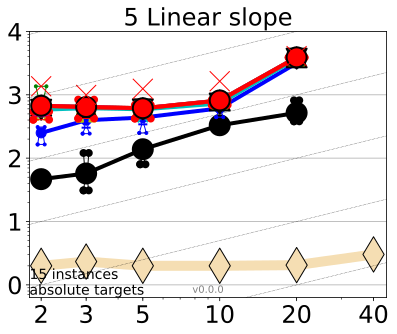
\includegraphics[width=0.266\textwidth]{ppfigdim_f010}\\
  \end{tabular}
  \vspace{-3ex}
   \caption{\label{fig:aRTgraphs}
   \bbobppfigdimlegend{$f_1$ and $f_{24}$}
  }
  \end{figure*}
  %
  The results of the comparison are shown in Figure \ref{fig:aRTgraphs},
  which follow the classical BBOB 2009 format, which includes the amount
  of effort devoted to finding a certain fitness level and time needed
  to do it. The EvoSpace and KafkEO results are shown side by side, only
  for the sake of comparison, since we are only interested for the time
  being in the baseline performance of the proof of concept.

The results obtained show that the basic Genetic Algorithm implemented
  in KafkEO does not perform
  very well against the testbed, specially when compared against other nature
  inspired algorithms like PSO or other hybrid approaches \cite{hansen2010bbob}.
  However, both implementations, shown side by side, reach similar results with the same
  effort; and the results in this case have been obtained with fewer
  parameters, with out the need to specify an initial pool size and
  % parameter, simply the number of initial populations, and no tweaking
  without tuning the evolutionary algorithm parameters.

  This is a problem that pool-based algorithms have: we need to
  specify the initial number of individuals to place in the pool and have the
  burden of always keeping a minimum number of individuals in the pool. This
  is not the case in KafkEO, because there is no need to have a
  repository for the population. However, population size and the number
  of generations turned in by every instantiation of the functions have
  to be tuned, which is something that will have to be left as future
  work.


  \section{Conclusions}
  \label{sec:con}

  This paper is intended to introduce a simple proof of concept of a
  serverless implementation of an evolutionary algorithm. The main
  problem with this algorithm, shared by many others, is to turn
  something that has state (in the form of loop variables or anything
  else) into a stateless system. In this initial proof of concept we have
  opted to create a stateful {\em mixer} outside the serverless (and
  thus stateless) platform to be able to perform {\em
    migration} and mixing among populations. A straightforward first step
  would be to parallelize this service so that it can respond faster to
  incoming evolved populations; however, this scaling up should be done
  by hand and a second step will be to make the architecture totally
  serverless by using functions that perform this mixing in a stateless
  way. This might have the secondary effect of simplifying the messaging
  services to a single topic, and making deployment much easier by
  avoiding the desktop or server back-end we are using now for that
  purpose.

  The proof of concept is a good adaptation of an evolutionary algorithm
  to the serverless architecture, with a performance that is comparable,
  in terms of number of evaluations, to pool-based architectures. Even
  if results right now are not competitive, the scalability of the
  architecture and also the possibilities it offers in terms of tuning
  parameters for the algorithm, even using heterogeneous functions
  tapping the same {\em topic} (channel), offer the chance of improving
  running time as well as the algorithm itself in terms of number of
  evaluations. This is an avenue that we will explore in the near
  future. The whole set of experiments, done in the cloud with a desktop
  component, took more than running a single desktop experiment using
  EvoSpace. However, scaling was lineal with problem difficulty, which
  at least mean that we are not adding an additional level of complexity
  to the algorithm and might indicate that horizontal or vertical
  scaling would solve the problem. This kind of scaling also indicates
  that the stateful part, run in a desktop, has not for this problem
  size become a bottleneck. Even so, we consider that it is essential to
  create an algorithm architecture that will be fully serverless and,
  thus, stateless.

  Other changes will go in the direction of testing the performance of
  the system and computing the cost, so that we can increase the former
  without increasing the latter. Since there is room for increasing
  parallelism, we will try different ways of obtaining better
  algorithmic results by making a parameter sensitivity analysis,
  including population size, length of evolution runs, and other
  algorithmic parameters.  Once those algorithmic baselines have been set, we will experiment
  with different metaheuristics such as particle swarm optimization, or
  even try for heterogeneous functions with different evolutionary
  algorithm parameters, with the purpose of reducing the number of
  parameters to set at the start.

\section*{Acknowledgments}

  This paper has been supported in part by
projects TIN2014-56494-C4-3-P (Spanish Ministry of Economy and
Competitiveness) and DeepBio (TIN2017-85727-C4-2-P)

  \bibliographystyle{splncs03}
  \bibliography{serverless}

  \end{document}

